\documentclass[10pt]{article}
\usepackage[utf8]{inputenc}

\usepackage{fullpage}
\usepackage{amsmath,amssymb, amsfonts,amsthm, enumerate}
\usepackage{mathbbol}
\usepackage{graphicx}

\usepackage{booktabs}  % nice looking tables
\usepackage{numprint}
\npdecimalsign{.}
\nprounddigits{2}

% these are compressed lists to help fit into a 1 page limit
\newenvironment{enumerate*}%
  {\vspace{-2ex} \begin{enumerate} %
     \setlength{\itemsep}{-1ex} \setlength{\parsep}{0pt}}%
  {\end{enumerate}}
 
\newenvironment{itemize*}%
  {\vspace{-2ex} \begin{itemize} %
     \setlength{\itemsep}{-1ex} \setlength{\parsep}{0pt}}%
  {\end{itemize}}
 
\newenvironment{description*}%
  {\vspace{-2ex} \begin{description} %
     \setlength{\itemsep}{-1ex} \setlength{\parsep}{0pt}}%
  {\end{description}}
  
\title{Stat 221 Problem Set 4}
\author{Albert Young and Marco Gentili}
\date{4 November 2014}

\begin{document}

\maketitle

\section{Question 1.1}
\[p(\lambda, \theta) = p(\theta,\mu) \propto \dfrac{1}{\lambda} = \dfrac{1}{\mu\theta}\]
To determine the induced distribution on $(N,\theta)$, we marginalize over $\mu$:
\begin{align*}
p(N, \theta)&=p(N|\theta)p(\theta)\\
&=\int_0^\infty p(N|\theta,\mu)p(\theta,\mu)\,d\mu\\ &\propto\int_0^\infty\dfrac{e^{-\mu}\mu^N}{N!}\dfrac{1}{\theta\mu}\,d\mu\\
&=\dfrac{1}{N!\theta}\int_0^\infty e^{-\mu}\mu^{N-1}\,d\mu\\
&=\dfrac{\Gamma(N)}{N!\,\theta}\\
&=\dfrac{(N-1)!}{N(N-1)!\,\theta}\\
&=\dfrac{1}{N\theta}
\end{align*}
\ldots giving us a nice polynomial form.


\section{Question 1.2}
No, $p(\lambda, \theta)$ is not a proper distribution. $\int_{0}^\infty \dfrac{1}{\lambda}\,d\lambda$ does not converge.

\section{Question 1.3}
\begin{align*}
Y_i &\sim Pois(\theta \cdot \mu)\\
p(Y_i|\theta, \mu) &= \dfrac{(\theta\mu)^{Y_i}}{(Y_i)!}\exp(-\theta\mu)\\
\log p(Y_i|\theta, \mu) &= -\theta\mu + Y_i\log(\theta\mu) + C
\end{align*}
where $C$ does not depend on $\theta$ or $\mu$. Calculating the Fisher Information:
\begin{align*}
\dfrac{\partial^2}{\partial\mu^2}\log p(Y_i|\mu, \theta) &= -\dfrac{Y_i}{\mu^2}\\
-E\left[\dfrac{\partial^2}{\partial\mu^2}\log p(Y_i|\mu, \theta)\right] &= \dfrac{\theta}{\mu}\\
\dfrac{\partial^2}{\partial\theta^2}\log p(Y_i|\mu,\theta) &= -\dfrac{Y_i}{\theta^2}\\
-E\left[\dfrac{\partial^2}{\partial\theta^2}\log p(Y_i|\mu,\theta)\right] &= \dfrac{\mu}{\theta}\\
\dfrac{\partial^2}{\partial \mu \partial \theta}\log p(Y_i|\mu,\theta) &= -1\\
-E\left[\dfrac{\partial^2}{\partial \mu \partial \theta}\log p(Y_i|\mu,\theta)\right] &= 1\\
det(I(\theta,\mu)) &= \dfrac{\theta}{\mu}\dfrac{\mu}{\theta} - 1 = 0\\
\end{align*}
So $p(\lambda, \theta)$ is not non-informative in the sense of Jeffreys.

\section{Question 1.4}
We ran MCMC for 10,000 iterations. We sampled $S=N\theta\sim Beta(\sum Y_i-1, Nn-\sum Y_i)$. Then, $N\sim Geom(\dfrac{\theta}{S})$. Our acceptance ratio is around 55\% for both datasets.\\
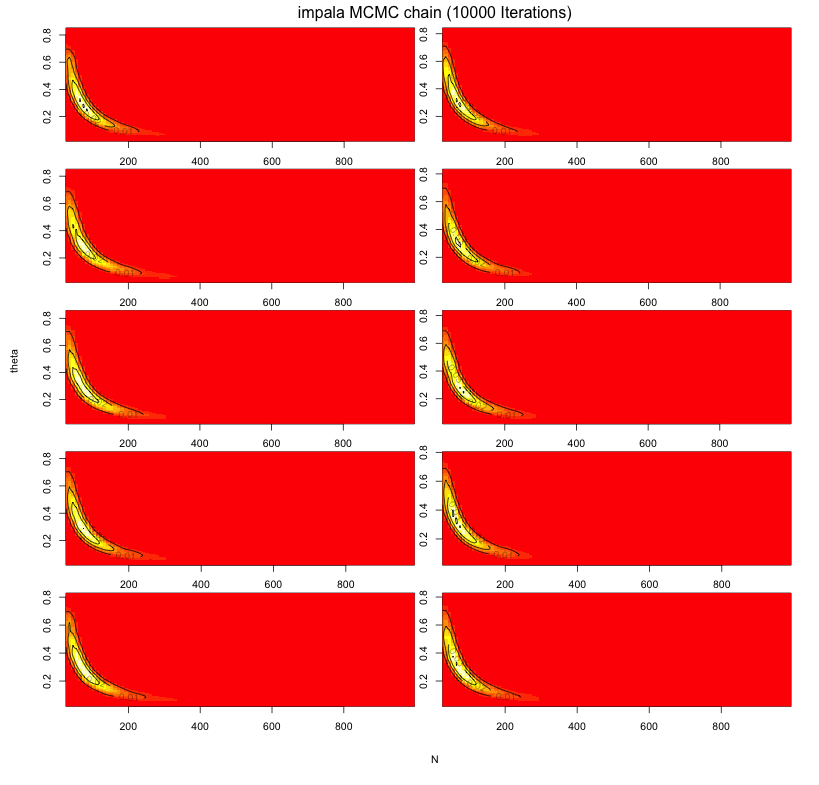
\includegraphics[scale=0.65]{impalamcmc.png}\\



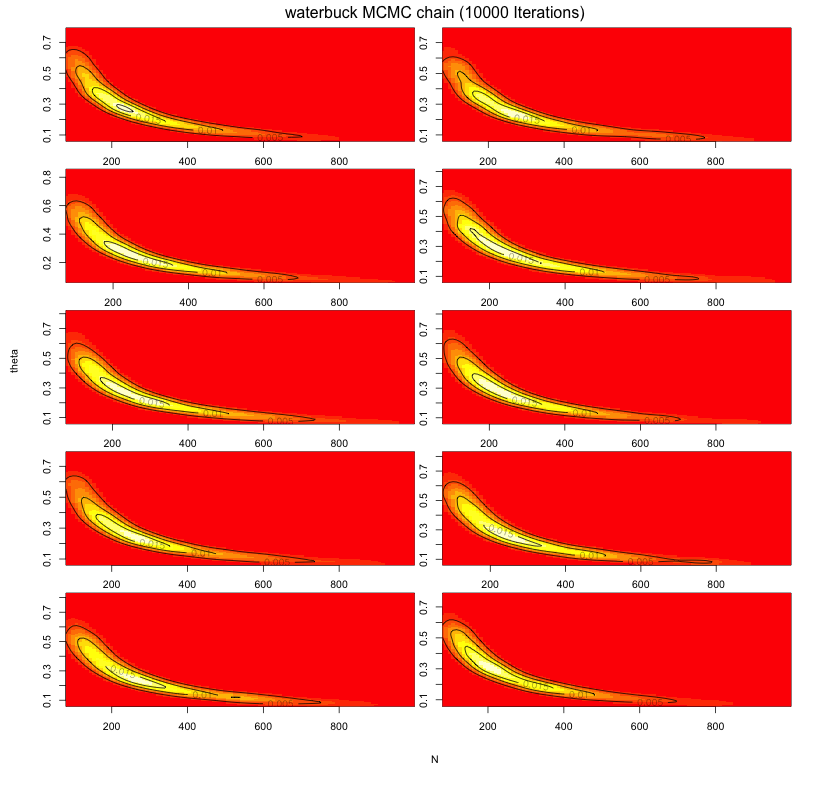
\includegraphics[scale=0.65]{waterbuckmcmc.png}\\
\section{Question 1.5}
\begin{align*}
p(N,\theta|Y) &= \dfrac{p(Y|N,\theta)p(N,\theta)}{\int p(Y|N,\theta)dNd\theta}\\
p(N|Y) &= C\int_0^1 p(Y|N,\theta)p(N, \theta)d\theta\\
&=\dfrac{C}{N}\prod_{i=1}^n\dbinom{N}{Y_i}\int_0^1\theta^{\sum{Y_i}-1}(1-\theta)^{Nn-\sum Y_i}d\theta\\
&=\dfrac{C}{N}\prod_{i=1}^n\dbinom{N}{Y_i}\dfrac{\Gamma(\sum{Y_i})\Gamma(Nn-\sum Y_i+1)}{\Gamma(Nn+1)}\\
&=\dfrac{C}{N}\prod_{i=1}^n\dbinom{N}{Y_i}\left(\dfrac{\sum Y_i (\sum Y_i - 1)! (Nn - \sum Y_i)!}{(Nn)!\sum Y_i}\right)\\
&=\dfrac{C}{N}\dfrac{1}{\dbinom{Nn}{\sum Y_i} \sum Y_i}\prod_{i=1}^n\dbinom{N}{Y_i}\\
\sum_N p(N|Y) &= \sum_N\left( \dfrac{C}{N}\left(\dfrac{1}{\dbinom{Nn}{\sum Y_i} \sum Y_i}\right)\prod_{i=1}^n\dbinom{N}{Y_i}\right) = \dfrac{1}{C}
\end{align*}
Taking advantage of  $\theta^{\sum{Y_i}-1}(1-\theta)^{Nn-\sum Y_i}\sim Beta(\sum{Y_i},Nn-\sum Y_i+1)$.
$\dfrac{1}{C}$ is our normalizing constant.

We can't sum can't sum across $N$s to infinity so we have an upper cutoff $N_{max}$. Summing from $N=1$ to $N_{max}=e^{15} = 3269017$, we obtain a normalizing constant of $4.687545e-08$ for the impala data and $6.651808e-08$ for the waterbuck data.\\


\pagebreak
IMPALA DATA:\\
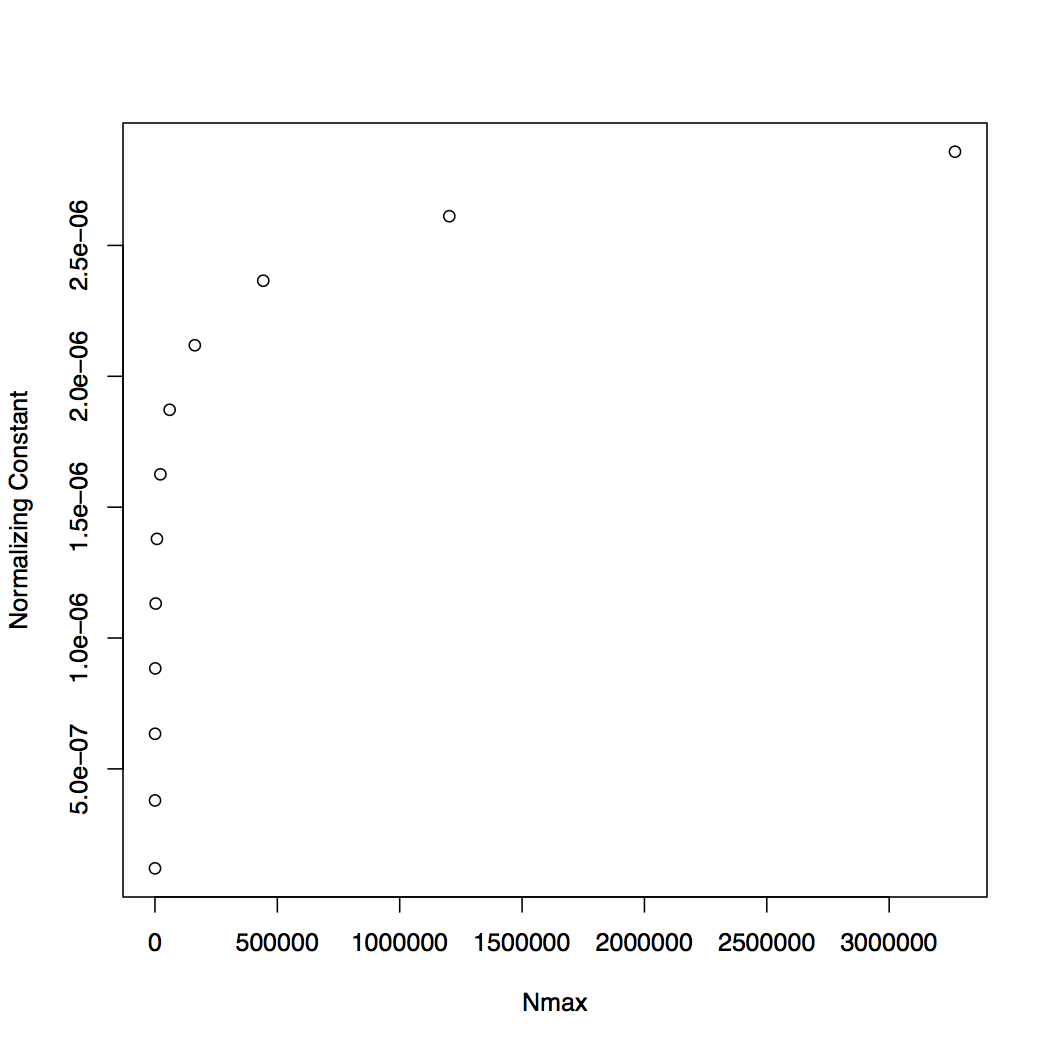
\includegraphics[scale=0.75]{impalanormc.png}\\
\pagebreak
WATERBUCK DATA:\\
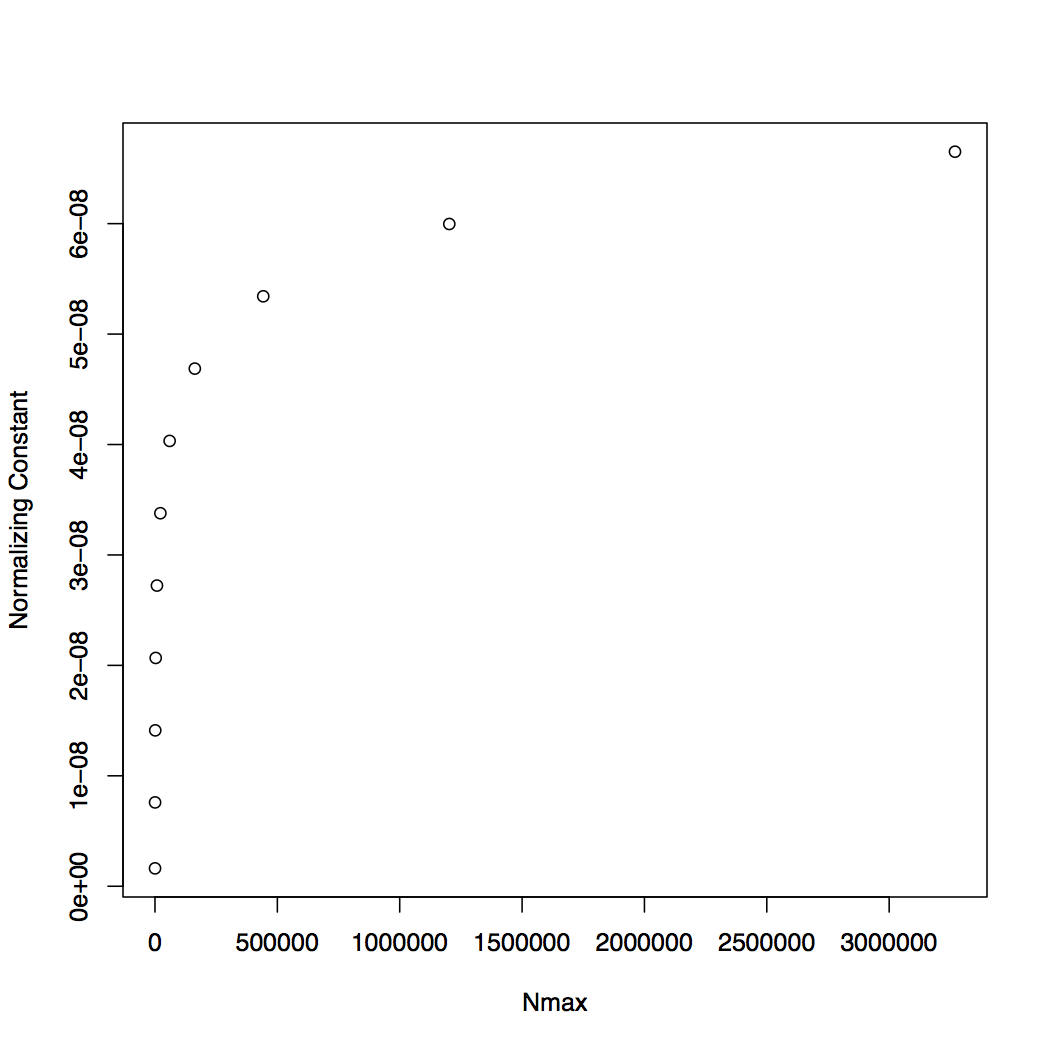
\includegraphics[scale=0.75]{waterbucknormc.png}

\section{Question 1.6}
For the posterior probability that $N>100$, we obtained $.4443$ for the impala and $.9734$ for the waterbuck datasets, respectively.

The posterior analytics for IMPALA for 10 chains:\\
\begin{table}[h]
\begin{tabular}{llll}
mean of N & theta mean        & N sd             & theta sd          \\
562.6458  & 0.277963067889716 & 7734.6927528985  & 0.192755573974767 \\
606.7675  & 0.283222893222428 & 10994.9857642763 & 0.196222534258168 \\
529.8685  & 0.266034858270702 & 7004.90443723719 & 0.192651141217575 \\
310.7725  & 0.271150421612974 & 1604.4739139038  & 0.190313579905066 \\
299.0939  & 0.273036193335137 & 1470.02884024835 & 0.19483950133021  \\
364.636   & 0.275585642568672 & 4773.39335350804 & 0.188345061657908 \\
343.8988  & 0.275394386473951 & 2230.53458126306 & 0.194183567944313 \\
237.8746  & 0.281194063195724 & 748.629962102009 & 0.189712764848506 \\
249.0048  & 0.275086596973311 & 817.206296102764 & 0.189637013466521 \\
284.8015  & 0.279820325894997 & 1368.82568191589 & 0.192675396725995
\end{tabular}
\end{table}\\
The posterior analytics for WATERBUCK for 10 chains:\\
\begin{table}[h]
\begin{tabular}{llll}
N mean    & theta mean        & N sd             & theta sd                  \\
1808.7721 & 0.252534661435681 & 34864.3725616162 & 0.176124672730363 \\
3650.5406 & 0.230168067949625 & 64985.6590189971 & 0.176697277434169 \\
1733.8773 & 0.23790001011818  & 21642.9758183035 & 0.179266390848925 \\
1032.0534 & 0.238284848648184 & 4478.15529903069 & 0.174011580648649 \\
1761.6458 & 0.230391570960453 & 17656.2429029136 & 0.173322859129494 \\
834.8959  & 0.245838955571044 & 3210.58914284086 & 0.17751790617653  \\
2060.0502 & 0.236212304212799 & 24943.6691832118 & 0.176469790227135 \\
1592.9866 & 0.241322634819646 & 12971.1625989168 & 0.179918973072355 \\
1358.5298 & 0.238231696529153 & 11611.0746579799 & 0.174486573154321 \\
1560.9429 & 0.242356503626048 & 10597.3512770243 & 0.176531597736815
\end{tabular}
\end{table}
\end{document}
